\documentclass{beamer}

\usepackage{babel, graphicx}
\usepackage{tikz}
\usepackage{subfig}
\usepackage[T1]{fontenc}

\usetheme{Frankfurt}

\title{ \large{Rock-Paper-Scissors} \\
        \small{ML 2023/2024}}

\author{
    Maksymilian Wiśniewski \and
    Michał Mękarski \\ \and
    Patryk Maciąg  \and
    Stanisław Reda
}

\date{}

\titlegraphic{
\centering
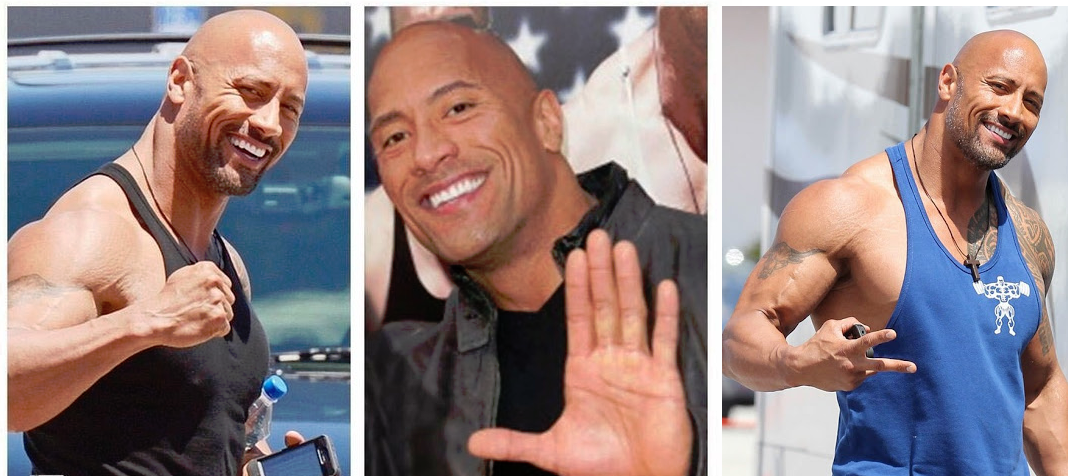
\includegraphics[height=1in, width=3in]{images/rock.png}
}

\begin{document}

\maketitle

\section{Main Goal}

\begin{frame}
    \frametitle{Main Goal}
    \begin{itemize}
        \item We decided to focus on the classification of images.

        \item Our main goal is to classify the gesture in the photo as one of the three movements from the "Rock-Paper-Scissors" game with best possible accuracy.
    \end{itemize}
\end{frame}

\section{Data}

\begin{frame}
    \frametitle{Data}
    On Kaggle we have many datasets with photos to use, such as:
    \begin{itemize}
    \item \href{https://www.kaggle.com/datasets/drgfreeman/rockpaperscissors}{Rock-Paper-Scissors Images}

    \item \href{https://www.kaggle.com/datasets/manasdalakoti/rock-paper-scissors-0528}{Rock Paper Scissors 0528}

    \item \href{https://www.kaggle.com/datasets/sanikamal/rock-paper-scissors-dataset}{Rock Paper Scissors Dataset}

    \item \href{https://www.kaggle.com/datasets/anirudhabhagwat/rock-paper-scissors-images}{rock paper scissors images}

    \item \href{https://www.kaggle.com/datasets/yash811/rockpaperscissors}{rock-paper-scissors}

    \end{itemize}
    \begin{figure}
    \centering
    \subfloat{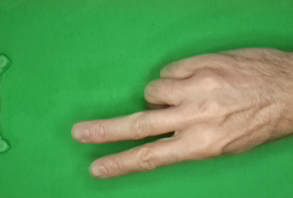
\includegraphics[width=0.2\textwidth]{images/nozyce.png}\label{fig:img1}}\hfill
    \subfloat{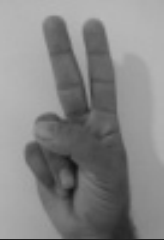
\includegraphics[width=0.2\textwidth]{images/nozyce2.png}\label{fig:img2}}\hfill
    \subfloat{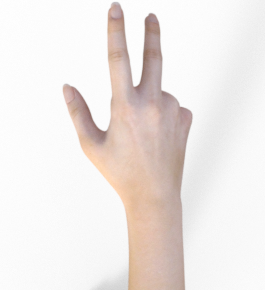
\includegraphics[width=0.2\textwidth]{images/nozyce3.png}\label{fig:img3}}\hfill
    \subfloat{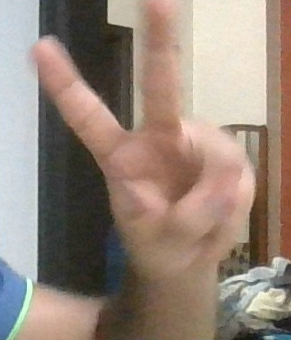
\includegraphics[width=0.2\textwidth]{images/nozyce4.png}\label{fig:img4}}\hfill
    \subfloat{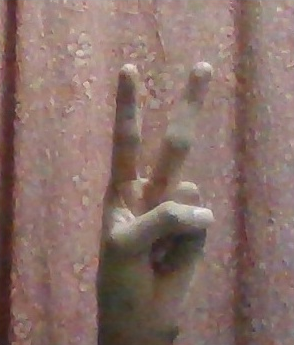
\includegraphics[width=0.2\textwidth]{images/nozyce5.png}\label{fig:img5}}
    \end{figure}
\end{frame}

\section{Methods}

% \begin{frame}
%     \frametitle{Methods}

%     \begin{itemize}
%         \item KNN

%         \item Clustering
%         \item K-means

%         \item Naïve Bayes

%         \item Logistic Regression

%         \item Decision trees
%         \item Random Forest

%         \item Support Vector Machine
%         \item Gradient Boosting

%     \end{itemize}

% \end{frame}

\begin{frame}
  \frametitle{Clear dataset (no augmentation)}

  \begin{table}
    \centering
    \begin{tabular}{|c|c|c|}
      \hline
      \textbf{Model} & \textbf{No PCA} & \textbf{PCA} \\
      \hline
      KNN & 91.32\% & 91.55\% \\
      \hline
      Decision tree & 84.02\% & 73.97\% \\
      \hline
      Random Forest & 94.74\% & 90.18\% \\
      \hline
      XGBoost & N/A & 91.09\% \\
      \hline
      Support Vector Machine & 68.72\% & 68.03\% \\
      \hline
    \end{tabular}
  \end{table}

\end{frame}

\begin{frame}
  \frametitle{Augmented dataset}
\centering
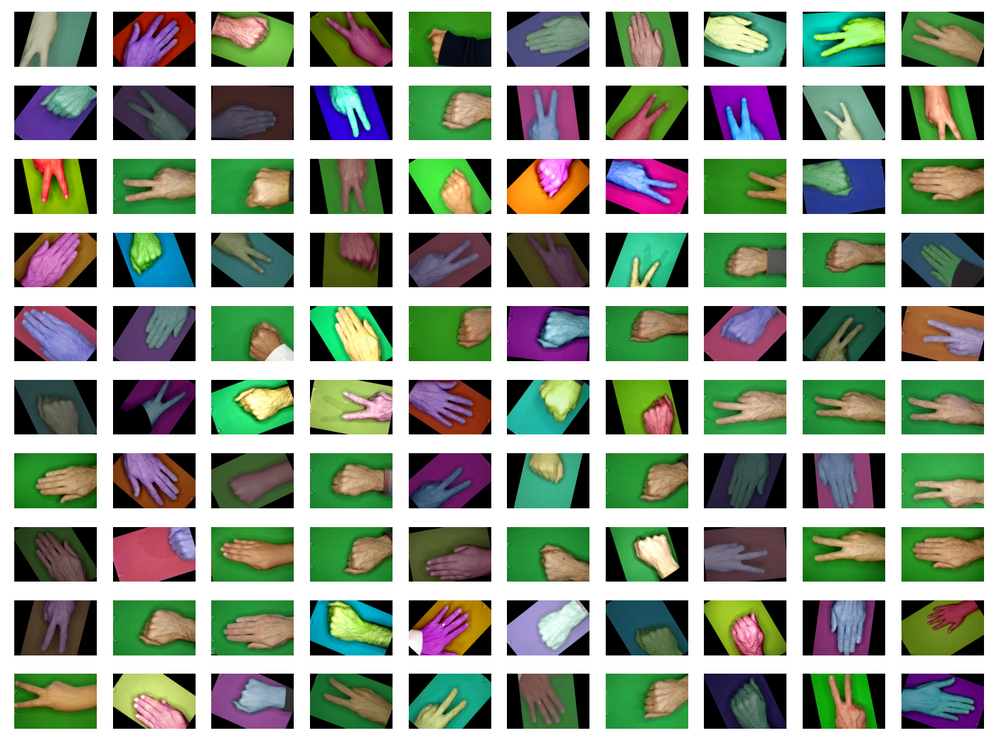
\includegraphics[height=3in, width=4.2in]{images/augmented.png}
\end{frame}

\begin{frame}
  \frametitle{Augmented dataset}

  \begin{table}
    \centering
    \begin{tabular}{|c|c|c|}
      \hline
      \textbf{Model} & \textbf{No PCA} & \textbf{PCA} \\
      \hline
      KNN & 68.59\% & 69.78\% \\
      \hline
      Decision tree & 64.93\% & 58.59\% \\
      \hline
      Random Forest & 86.41\% & 76.92\% \\
      \hline
      XGBoost & N/A & 87.26\% \\
      \hline
      Support Vector Machine & 43.86\% & 45.06\% \\
      \hline
    \end{tabular}
  \end{table}

\end{frame}

\begin{frame}
  \frametitle{What next?}

    \begin{itemize}
        \item Preprocessing

        \item Feature extraction

        \item Extened training set by self-made photos of hands.

    \end{itemize}

    \centering
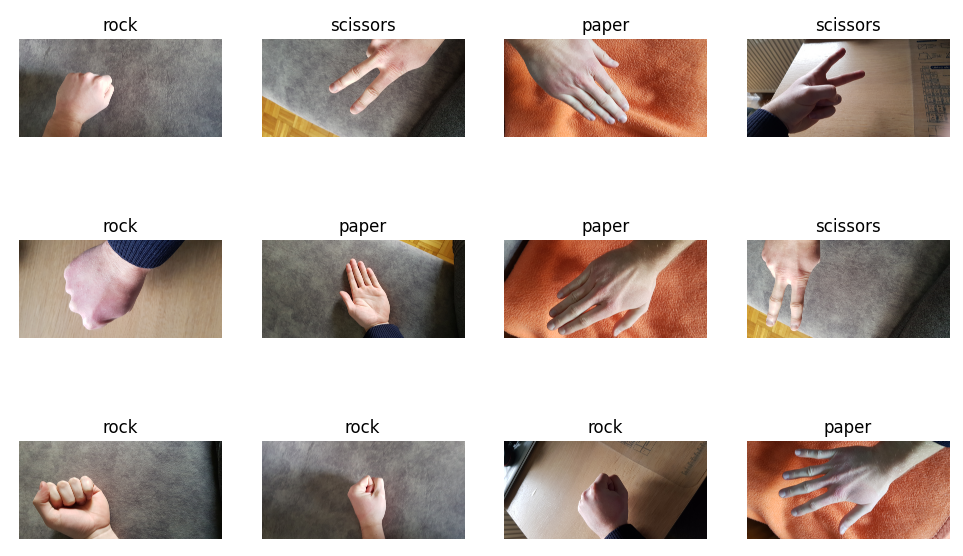
\includegraphics[height=2in, width=3in]{images/real.png}

\end{frame}

\end{document}
